%!TEX root = ../../Paper.tex

\chapter{Use Cases}
\label{cha:use-cases}

\section{General Use Cases}
\label{sec:general-use-cases}


\section{Stock Market Prediction}
\label{sec:stock-market-prediction}
Predicting the trends of the stock market is hugely important for today's businesses. However, a precise prediction seems to be very complex since the prices "follow a random walk pattern and cannot be predicted with more than 50 percent accuracy" \cite[1]{bollen2011twitter}. However, Twitter can predict the stock market if the right Tweets are analyzed \cite{bollen2011twitter}. The company \textbf{Dataminr} scans Twitter for relevant messages characterized by "the right combination of language, context and location" to detect "breaking- and money-making-news" \cite{alcorn2013stockmarket}.

\begin{figure}[H]
  \centering
        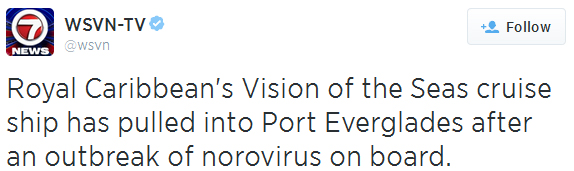
\includegraphics[width=25em]{tweet_norovirus}
  \caption[Tweet announcing the outbreak of norovirus on March 8, 2013]{Tweet announcing the outbreak of norovirus on March 8, 2013 \cite{wsvnnorovirus2013}}
  \label{fig:use_case_stock_market}
  \vspace{-1.3em}
\end{figure}

In 2013, a cruise ship of Royal Carribean arrived with more than 100 passengers sick with norovirus. A news agency published a Tweet announcing the outbreak of norovirus (see figure \ref{fig:use_case_stock_market}). Dataminrs' clients got this news two minutes later, but 48 minutes earlier than others, because their algorithm "found that words in the tweet had some resemblance to tweets in the past that had turned out to be newsworthy". According to Dataminr, the alert saved money of at least one client, due to a falling share price. Besides financial clients, also government organizations are interested in Dataminrs' Twitter analysis \cite{alcorn2013stockmarket}.

\section{Flu Trend Prediction}
\label{sec:flu-trend-prediction}
Seasonal influenza is responsible for millions of illnesses and up to 500 thousand deaths per year. Therefore, it is known as a major health issue all over the world. An early detection of epidemics would reduce the significant effect of pandemic and seasonal influenza. The project \textbf{Google Flu Trends} aims to monitor flu cases in real time and thereby predict flu trends by analyzing social datasets \cites{Google09detection}[1]{Tech22014}.

The Google-researchers identified 45 keywords with a strong correlation to the appearance and spread of seasonal flu \cites{Weber2014}. With these keywords, it should have been possible to get information about the spread of flu or even the start of a new wave of influenza \cites{Weber2014}{Tech22014}{gft2014}. Figure \ref{fig:use_case_gft} visualizes the flu activity in the United States.

\begin{figure}[H]
  \centering
        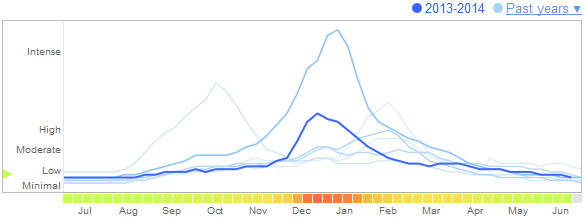
\includegraphics[width=30em]{gft_us}
  \caption[Flu activity in the United States]{Flu activity in the United States \cite{gft2014}}
  \label{fig:use_case_gft}
  \vspace{-1.3em}
\end{figure}

However, the project overestimated peak flu cases in the past two years and even failed to detect the H1N1\footnote{\url{http://www.cdc.gov/h1n1flu/qa.htm} \accessednote} pandemic in 2009 \cites{Tech22014}. Figure \ref{fig:use_case_gft_comparison} illustrates the estimated flu activity compared to official data. The overestimation might have happened because of not having investigated data validity or reliability \cites{Weber2014,Tech22014}. 

\begin{figure}[H]
  \centering
        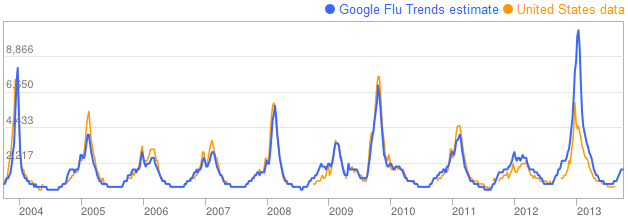
\includegraphics[width=30em]{gft_comparison_real_data}
  \caption[Google Flu Trend estimation compared to real data]{Google Flu Trend estimation compared to the real data\footnotemark \cite{gftcomparison2014}}
  \label{fig:use_case_gft_comparison}
\end{figure}
\footnotetext{delivered by U.S. Centers for Disease Control \url{http://www.cdc.gov/} \accessednote}

Ryan Kennedy, a professor at the University of Houston stresses, that "Google Flu Trend is an amazing piece of engineering and a very useful tool, but it also illustrates where Big Data analysis can go wrong" \cites{Tech22014}. Kennedy concludes that more accurate results could have been achieved by combining Big Data analysis with more traditional methodologies \cites{Tech22014}.